% TFF-Title: Directed textbook graph
% TFF-Family: graph
% TFF-Tags: graph, directed-network, curved-edges, weights, textbook
% TFF-Description: Compact directed graph with asymmetric weighted links and clean bend separation.
% TFF-Origin: https://texample.net/tkz-berge/
% TFF-License: CC BY-SA 4.0
% TFF-Attribution: Adapted from Alain Matthes' tkz-berge example on TeXample.net
\documentclass[tikz,border=7pt]{standalone}
\usetikzlibrary{arrows.meta}
\begin{document}
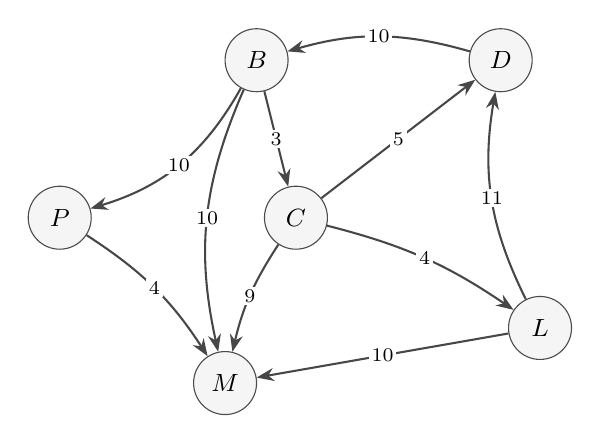
\begin{tikzpicture}[
  vertex/.style={circle,draw=black!70,fill=gray!8,minimum size=8mm,font=\small},
  arc/.style={-{Stealth[length=2.2mm]},draw=black!72,line width=.75pt},
  weight/.style={fill=white,inner sep=1pt,font=\scriptsize}
]
\node[vertex] (P) at (0,0) {$P$};
\node[vertex] (B) at (2.5,2.0) {$B$};
\node[vertex] (C) at (3.0,0.0) {$C$};
\node[vertex] (M) at (2.1,-2.1) {$M$};
\node[vertex] (D) at (5.6,2.0) {$D$};
\node[vertex] (L) at (6.1,-1.4) {$L$};

\draw[arc] (P) to[bend left=12] node[weight] {4} (M);
\draw[arc] (B) to node[weight] {3} (C);
\draw[arc] (C) to[bend right=10] node[weight] {9} (M);
\draw[arc] (C) to node[weight] {5} (D);
\draw[arc] (C) to[bend left=10] node[weight] {4} (L);
\draw[arc] (B) to[bend right=18] node[weight] {10} (M);
\draw[arc] (D) to[bend right=16] node[weight] {10} (B);
\draw[arc] (L) to[bend left=18] node[weight] {11} (D);
\draw[arc] (L) to node[weight] {10} (M);
\draw[arc] (B) to[bend left=22] node[weight] {10} (P);
\end{tikzpicture}
\end{document}
